\documentclass[11pt]{article}

\usepackage{float}
\usepackage{graphicx}
% \usepackage{natbib}
\usepackage{amsmath}
\usepackage{geometry}
\usepackage{apacite2}

\setcounter{tocdepth}{2} 

\geometry{
 body={6.5in,9in},
 left=1in,
 right=1in,
 bottom=1in,
 top=1in
}

\title{Learning Mathematics in a Visuospatial Format\\ Supplemental Online Material}
\author{BLINDED}
% \author{David Barner, George A. Alvarez, Jessica Sullivan, Neon Brooks, \\ Mahesh Srinivasan, and Michael C. Frank} 
\date{}

\begin{document}
\maketitle
\tableofcontents
\newpage

\section{Tasks}

\subsection{Computerized Tasks}

For all computerized tasks, participants were familiarized with the task in a classroom setting at the beginning of each testing session. Example stimuli were presented on a large screen. The goal of each task was explained to students, as well as the keys they would need to press to respond. The tasks were explained by an experimenter in English, and by the classroom teacher in Hindi and Gujarati. In this familiarization session, children decided on answers as a group and some children were selected to demonstrate entering the responses. Training occurred 1 -- 3 days before testing. 

Computer testing was conducted in two separate testing blocks: on the first block, participants were tested on spatial and verbal working memory. On a later day, they were given a second computer testing session with the number comparison task, and (in Years 1 -- 3) a number quantity estimation task, not analyzed in the current study due to the lack of baseline Year 0 data. On the day of testing, participants came to the testing room in groups of 8 -- 16 and first received a small-group refresher during which the task was again explained.  Participants were asked to respond to sample questions both as a group and individually. Feedback was provided. Children were then each seated at their own computer with barriers preventing them from seeing the computers to either side of them. Children wore headphones for all tasks. Experimenters circulated throughout the room to make sure all children understood the tasks and stayed focused.

\subsubsection{Number Comparison}

In the Number Comparison task, children were presented with a pair of dot arrays on each trial and were asked to choose the larger of the two arrays. 

{\it Stimuli.} Two arrays of dots were presented simultaneously on each trial. Arrays were black dots on a gray background, separated by a black line running down the middle of the screen. Total surface area of the dots was controlled for 50\% of the trials and item size for the other 50\% \cite{dehaene2005}.

{\it Procedure.} The task was self-paced: participants pressed a space-bar to display the next array of dots. Two short beeps delivered via headphones preceded the presentation of the arrays. Arrays were visible for 1 second, and were followed by a mask of random noise for 300 ms. Participants indicated which side had more dots by pressing either a right arrow or left arrow taped onto the ``Z'' and ``M'' keys on the keyboard. Feedback was provided.

Children's performance was measured across blocks of 8 trials. For each block, participants were tested on one specific numerical ratio (e.g., 4:5). Within each block, the numerical magnitudes of the arrays varied widely (e.g., 8 vs. 10; 120 vs. 150), and the correct answer was on the left for 50\% of the trials. A participant was determined to have succeeded on a block if (s)he correctly chose the larger set on 6 of 8 trials. Trials were pseudo-randomly ordered such that a response pattern of alternating ``left'' and ``right'' responses could not lead to success on that block. Success on any given block was, therefore, impossible for any child who was responding solely based on non-numerical parameters, or for any child who consistently provided ``left'' responses, ``right'' responses, or alternating responses. 

The task was adaptive, such that success on a given block of 8 trials determined the difficulty of the ratio presented on the next block. All participants started at a 4:5 ratio. Failure on a given block sent participants to the next easiest ratio (e.g., 3:4), while success sent participants to the next hardest ratio (e.g., 5:6). Possible ratios ranged from 1:5 to 13:14.

{\it Scoring.} For each child, we used all trials they completed to estimate their Weber fraction via the maximum likelihood algorithm given in \citeA{halberda2008}.

\subsubsection{Spatial Working Memory} 

In the Spatial Working Memory Task, participants compared two sequences of successive locations in a grid, with the length of the sequences determined by an adaptive staircase procedure. 

{\it Stimuli.} On each trial, participants were presented with a $5x5$ array of 25 circles, arranged in a grid in the center of the screen. After the start of the trial, a sequence of circles (with sequence length depending on the level of the trial) would fill with yellow and then become empty again (such that only one circle was filled at any time). Each time a filled circle appeared, participants heard an attention-getting noise through their headphones. After the yellow dots had all appeared and disappeared, the subjects saw a series of blue dots appear and disappear in the same manner. The blue dots would either appear in the same locations as the yellow dots, or the position of one member of the sequence would be altered by one space in the grid. 

The participants' task was to determine whether the two sequences were identical. Two short beeps delivered via headphones preceded the presentation of the arrays. Participants responded by pressing keys marked ``S'' for same and ``D'' for different. After receiving feedback on their answer, participants were prompted to press the space bar to begin the next trial. 

{\it Procedure.} Each session began with 10 practice trials that increased in difficulty from 1 to 3 circles. Difficulty in the main trial block of 24 trials was adaptive, such that success on a given trial determined the difficulty of the trial presented on the next block. If a participant got two successive trials correct, the level of difficulty of the next trial would increase by one; with one trial incorrect, the level would decrease by one. 
 
{\it Scoring.} For each child, we averaged the difficulty level of all of their experimental trials to find their spatial working memory score. We determined empirically that, given the relatively short length of the task, this method maximized year-to-year correlations in our data. 

\subsubsection{Verbal Working Memory}

The Verbal Working Memory task was designed to be as closely matched to the spatial working memory task as possible, with sequences of syllables substituted for sequences of locations. 

{\it Stimuli.} On each trial, subjects were presented with a blank gray screen. Two short beeps delivered via headphones preceded the delivery of a sequence of syllables. All syllables were recorded by a native Gujarati speaker, using consonants and vowels that are common to English, Gujarati, and Hindi. A smiley-face icon appeared on the left side of the screen while each syllable in the sequence was presented. This first sequence of syllables were followed by a second set of two beeps, and a second sequence of syllables, with a smiley-face icon appearing on the right side of each screen as each syllable was presented. 

As in the spatial working memory task, participants reported whether the two sequences were identical or not by pressing the keys marked either ``S'' for same or ``D'' for different on their keyboard. The task was self-paced: participants pressed the space-bar to display the next trial. The task was adaptive in exactly the same manner as the spatial working memory task. It also began with 10 practice trials before proceeding through 24 experimental trials.

{\it Procedure and scoring.} Procedures and scoring were identical to the spatial working memory task.

\subsection{Paper and Pencil Tasks}

All paper tasks were administered in a group setting, and children recorded their own responses using their pencils. At each administration, the task was explained first by an experimenter in English, and then by a classroom teacher in Hindi, Gujarati, and English. All tasks except the Growth Mindset and Math Anxiety measures were timed (time limits described below). Erasers were provided, and students were permitted to change their answers until time was up. Classroom teachers and experimenters were available to answer questions about the format of the task. Students who finished early were encouraged to check their work. 

Paper and pencil tasks were given in 2 - 3 separate sessions each year to prevent fatigue. For years 1 -- 3, at the end of each year's testing period, students in the abacus group completed a fourth battery of abacus-specific tasks as a manipulation check. Finally, in year 3, all students completed the growth mindset and math anxiety questionnaires, which measured whether the intervention had changed their attitudes toward mathematics and achievement.

\subsubsection{Place Value}

The Place Value task tested conceptual understanding of the place value decomposition of multi-digit numbers.

{\it Stimuli.}  The test sheet consisted of 11 test problems and 1 example problem. For each problem, there was a box containing an addition problem with one addend missing (e.g., ``4000 + \underline{\hspace{1cm}} + 400 + 6 = 4456)''. This box was labeled in both English and Gujarati: “Fill in the blank/Khali jagyao puro.” On the right side of the page was a space to write answers labeled “Answer/Javaab.” Critically, adding the digits was not necessary to solving this problem -- participants could solve each problem without computing the sums if they understood place value. Addends were pseudo-randomly ordered, and each addend contained only one non-zero digit (e.g., 4000 was a possible addend; 4050 and 4500 were not). 

Trials varied in difficulty: the missing addend was in the 1s place on 4 trials, the 10s place on 5 trials, the 100s place on 1 trial, and the 1000s place on 1 trial The example problem was a simple addition problem containing the question ``3 + \underline{\hspace{1cm}} = 4'' and the answer ``1''. Each year, the specific problems changed to prevent familiarity effects, but the example problem remained the same, as did the constraints on problem properties. 

{\it Procedure.} Participants were given 4 minutes to answer as many questions as possible. The goal of the short time limit was to prevent participants from being able to solve all 11 problems by computing the relevant sums---participants who recruited arithmetic operations were unlikely to be able to finish all 11 problems correctly, while those who used place value knowledge could theoretically complete the task in mere seconds. Participants were told to figure out the missing addend as quickly as possible. Possible scores ranged from 0 -- 11 each year, except for in year 3, when a typo required the exclusion of one problem.

\subsubsection{Arithmetic} 

Our in-house arithmetic task tested children's speed and accuracy in solving basic arithmetic problems.

{\it Stimuli.} The test sheet consisted of 48 test problems. For each problem, there was a box containing the math problem to be solved. This box was labeled in both English and Gujarati: ``Question/Savaal.'' On the right side of the page was a space to write answers labeled ``Answer/Javaab.'' There was also a place for children to write down their work. 

There were 16 addition problems, 16 subtraction problems, 8 multiplication problems, and 8 division problems. Trials varied in difficulty by varying the number of digits in each operand, the number of digits in each answer, and the number of carries required by each problem when solved via traditional arithmetic algorithms. For example, the easiest addition problem in year 3 was 3+5 (1-digit addends; 1-digit answer, no carrying), and the hardest in year 3 was 9,542+9,388 (4-digit addends; 5-digit answer, 3 carries). Each year, 40/48 trials were altered to include different addends (though trial difficulty remained constant across these changes) and 8 trials remained the same. 

{\it Procedure.} Participants were given 5 minutes to answer as many questions as possible. Participants were told to solve the problems as quickly as possible, and to try to get the right answer. 

\subsubsection{Ravens Progressive Matrices}

{\it Stimuli.} Children completed 1 or 2 sets of Ravens Progressive Matrices. Set A was administered in Years 0 -- 2, Set B in Years 2 -- 3, and Set C in Year 3. Each set had 12 questions. 

{\it Procedure.} Participants were told to solve the problems, and to record their answers on the response sheet. The task was explained by an experimenter in English and by the classroom teacher in Hindi and Gujarati. This test was administered in a group setting, and children recorded their own responses. There was a 10-minute time limit to complete each set. In years where two sets were administered, they were administered sequentially. 

\subsubsection{WJ-III}

{\it Stimuli.} The Woodcock Johnson Tests of Achievement (WJ-III) Calculation subtest.

{\it Procedure.} Participants were given a printout of the WJ-III Calculation subtest, and were told to try their hardest to solve as many problems as possible. Children were given 10 minutes to complete this task. 

\subsubsection{WIAT-III}

{\it Stimuli.} The Wechsler Individual Achievement Test (WIAT-III) Numerical Operations subtest.

{\it Procedure.} Participants were given a printout of the Numerical Operations subtest of the Weschler Individual Achievement Test and were told to try their hardest to solve as many problems as possible. Children were given 10 minutes to complete this task. 

\subsubsection{Mental Rotation}

We created a paper-and-pencil version of the \citeA{shepard1971} mental rotation task, using both the original stimuli and letter-based stimuli (which we expected would be significantly easier for children). 

{\it Stimuli.} Children were given booklets where each page contained two half-page mental rotation problems. Each problem included a single target figure (a letter or a Shepard-Metzler figure) presented above two test figures. One test figure was always the target figure after having been rotated in a 2-dimesional plane, and the second test figure was a mirror image of the first. The degree of rotation of the test figures increased over the course of the task, so that the early trials were relatively easy, and the later trials were relatively difficult.

{\it Procedure.} Students were told to circle the test figure that was a rotated version of the target figure. This task was preceded with a PowerPoint demonstration of the task that provided animated examples of how the correct test figure could be rotated in order to look identical to the target figure. Students completed two packets, each containing 36 items, at their own pace, with a time limit of 10 minutes per packet. The first packet consisted of letters, and the second packet consisted of Shepard-Metzler figures.

\subsubsection{Growth Mindset Questionnaire} 

The Growth Mindset questionnaire (adapted from \citeNP{dweck1999}) measured children's attitudes toward the malleability of their own intelligence and achievement. This questionnaire was only given in Year 3.

{\it Stimuli.} The questionnaire consisted of three example items, followed by six test items and three filler items. For each item, there was a statement, and children were asked to indicate the degree to which they agreed with that statement, on a six-point scale (1 = ``Strongly Disagree''; 6 = ``Strongly Agree''). The three example items were completed as a group, and were designed to give children practice with using the full extent of the scale. Two of the six test items presented children with statements about the malleability of intelligence (e.g., ``You are born with a certain level of smartness, and that cannot be changed very much''); these are the items analyzed in the main text.

Of the other four test items, two presented statements about the malleability of personality (e.g., ``The kind of person you are cannot be changed very much''), and the other two presented statements about the achievement of members of different castes (e.g., ``If you have a low caste, you can never get the same grades in school as a high caste child, even if you work hard''). These four test items were included as part of a distinct study, and so responses are not described here.  

{\it Procedure.} In contrast to the other paper tasks, participants were not given a time limit for completing the questionnaire. Instead, each item was read out loud and explained by the experimenter and teachers (in English, Hindi and Gujarati), and completed by students one-by-one. This was done to ensure that children could understand the statements that they were being asked to endorse or reject. 

\subsubsection{Math Anxiety Questionnaire}

The Math Anxiety questionnaire (adapted from \citeNP{ramirez2013}) measured the anxiety that children experienced when solving different kinds of math problems, and when participating in math class. This questionnaire was also only given in Year 3.

{\it Stimuli.} The questionnaire consisted of three example items, followed by sixteen test items. Each item presented children with a situation, and they were asked to indicate how nervous they felt about that situation, on a five-point scale (1 = ``Not nervous at all''; 5 = ``Very, very nervous''). Each point in the scale was also accompanied by a cartoon face that similarly ranged from happy to nervous. The three example items were completed as a group, and were designed to give children practice with using the full extent of the scale. The test items asked children how nervous they felt when solving math problems (e.g., ``How nervous do you feel when you have to solve 12 x 15?''), participating in math class (e.g., ``How nervous do you feel when you are in math class and you don't understand something?''), doing their homework, reading charts and clocks, and so on. 

{\it Procedure.} To ensure that children would understand each of the situations they were being asked to imagine, each item was read out loud and explained by the experimenter and teachers (in English, Hindi and Gujarati), and completed by students one-by-one. 

\subsection{Abacus-Only Tasks}

These tasks were administered on the last day of testing each year, and were only administered to the students who received the mental abacus intervention. These were designed to be manipulation checks (i.e., to ensure that abacus students had actually learned abacus; to test their math skill with the physical abacus). These tasks were only administered in Years 1 -- 3, because no child had received abacus training in Year 0.
 
\subsubsection{Abacus Decoding}

This task measured whether children could quickly and accurately decode the values shown on a physical abacus.

{\it Stimuli.} This task consisted of 23 problems and 1 example. For each problem, there was a schematic image of a 3-columned abacus, with the in-play beads drawn on the abacus (and out-of-play beads omitted from the abacus). The abacus is frequently drawn in this style in the materials used to teach students MA. Below each abacus was a box for writing out the value presented on the abacus. Each year, the specific problems changed to prevent familiarity effects, but the example problem remained the same, as did the constraints on problem properties. Problem difficulty was manipulated by changing the number of beads and the number of columns in play. 

In year 3, several students noticed small gaps between some of the beads and the bar on the abacus. While these gaps had been present in earlier years, no student had previously noticed them (this change likely indicates a growing awareness and familiarity with the abacus). For this reason, a subset of problems in year 3 were ambiguous, because beads that aren't touching the bar are technically out of play, and don't count toward the depicted number. For these two trials, responses that counted the ambiguous beads as ``in play'' or as ``out of play'' were considered correct. 

{\it Procedure.} Participants were told to complete as many problems as they could, as fast as they could, by reading off the quantity depicted on the abacus and writing it in the box. They were given 5 minutes to complete the task.

\subsubsection{Abacus Sums}

This task tested children's ability to use the physical abacus.

{\it Stimuli.} Stimuli were generated using the same criteria as the whole-group sums task (reported below), although the actual problems differed. Each year, the specific problems were also changed to prevent familiarity effects, but the example problem remained the same, as did the constraints on problem properties. In year 1, the task was 56 problems long (though no child finished all problems); in years 2 and 3, the task was 140 problems long. 

{\it Procedure.} Participants were told to complete as many problems as possible as accurately as possible, although they were required to use their physical abacus to do so. Participants were given 5 minutes to complete the task.

\subsubsection{Abacus Arithmetic}

This task similarly asked children to use their physical abacus to do arithmetic computations.

{\it Stimuli.} Stimuli were addition and subtraction problems, generated using the same criteria described in the whole group arithmetic task (but differing in answer and operands from the whole group task). In Year 1, there were 48 problems, and in Years 2 -- 3 there were 24. 

{\it Procedure.} Participants were told to complete as many problems as possible as accurately as possible, using their physical abacus.

\subsection{Other (Excluded) Tasks}

Each of these tasks was not included in our main analyses, either because its format changed substantially over the course of our study (making cross-year comparisons impossible) or because it was only tested during a subset of years. 

\subsubsection{Commutativity}

This task was 26 questions long, with 1 example question (7 = 7). Across all years, each trial consisted of a statement of equivalence (e.g., 4 - 2 = 2 - 4) and a place for the participant to indicate ``True'' or ``False.'' In year 0, participants could indicate their response by checking either the True/Saachu box or the False/Khotu box. This response format caused confusion among the students and was not repeated in later years. In years 1-3, children instead circled a smiley face labeled with True/Saachu to indicate that the equivalence was true, and a False/Khotu frowny face to indicate that the equivalence was not true.  Because task format changed between year 0 and year 1, we could not use these data to test hypotheses related to the longitudinal effect of our abacus intervention.

\subsubsection{Sums Task}

This task was 140 questions long, and consisted of addition problems that contained between 2 -- 6 two-digit addends. Problems varied in difficulty based on how many abacus moves each problem required, ranging from 2 moves to more than 20. Problems were presented vertically (e.g., each addend was directly below the previous addend), and participants could write answers below the problem. This task was not included in our main study, as it was added during Year 2, and was not designed to test hypotheses related to the longitudinal effect of our abacus intervention.

\subsubsection{Geometry}

This task consisted of 22 problems, and one example problem. For each problem, 6 gray boxes were presented, and each box contained a geometric shape. These problems were drawn from stimuli used in previous studies of intuitive geometry \cite{dehaene2006}. In each problem, 5 of the shapes shared a common property (e.g., were circles) and one differed (e.g., it was an oval). This task was not included in our main study, as it was only tested in Year 1, and was thus not useful to test hypotheses related to the longitudinal effect of our abacus intervention.

\subsubsection{Number Estimation}

In this task, participants viewed randomly generated arrays of dots, and had to guess how many dots they saw. They received no feedback, and completed as many trials as they could in 5 minutes. This task was not included in our main study, as it was only tested in Years 1 -- 3. Without baseline data from Year 0, it was not possible to include this task in our main analyses.

\section{Data Management}

\subsection{Exclusions}

As noted in the main text, participants who did not contribute data to each year were excluded from all analyses (n = 17). In addition, if a participant did not comply with experimental directions either by failing to answer all questions on a given task, or by providing non-permissible answers (like providing letters as responses to addition problems), their data for that task for that year were excluded (Year 0: WIAT n = 24; Place Value n = 1; Raven's n = 9; Years 1 -- 3: no exclusions).

\subsection{Data Entry}

For all computerized tasks, data were automatically recorded and analyzed using custom Matlab programs. For all paper tasks, raw data were entered by two experimenters (blind to condition), and any discrepancies were resolved by a 3rd experimenter (also blind to condition). In all cases, children were given credit for erasures and partial erasures, and answers were counted if they were entered onto the answer sheet or in the workspace provided. 

\subsection{Scoring}

Scores on each paper task were computed by dividing the total number of correct responses by the total number of responses possible. So, if a child provided 8 correct answers and 12 incorrect answers on a 24-question test, their score for that test would be 8/24 or .33. 

\section{Descriptive Statistics}

Tables \ref{tab:arith} -- \ref{tab:ans} give means, medians, and standard deviations for the main tasks included in our analysis. 

% latex table generated in R 3.0.2 by xtable 1.7-1 package
% Fri Dec 27 12:13:43 2013
\begin{table}[H]
\centering
\begin{tabular}{rrrrrrr}
  \hline
Year & $M_{control}$ & $M_{MA}$ & $median_{control}$ & $median_{MA}$ & $SD_{control}$ & $SD_{MA}$ \\ 
  \hline
  0 & 0.13 & 0.16 & 0.12 & 0.15 & 0.07 & 0.06 \\ 
    1 & 0.15 & 0.20 & 0.15 & 0.21 & 0.07 & 0.10 \\ 
    2 & 0.26 & 0.34 & 0.27 & 0.33 & 0.10 & 0.12 \\ 
    3 & 0.38 & 0.46 & 0.40 & 0.46 & 0.13 & 0.16 \\ 
   \hline
\end{tabular}
\caption{Descriptive statistics for arithmetic (proportion correct).} 
\label{tab:arith}
\end{table}
% latex table generated in R 3.0.2 by xtable 1.7-1 package
% Fri Dec 27 12:13:43 2013
\begin{table}[H]
\centering
\begin{tabular}{rrrrrrr}
  \hline
Year & $M_{control}$ & $M_{MA}$ & $median_{control}$ & $median_{MA}$ & $SD_{control}$ & $SD_{MA}$ \\ 
  \hline
  0 & 0.29 & 0.31 & 0.27 & 0.27 & 0.16 & 0.14 \\ 
    1 & 0.29 & 0.31 & 0.18 & 0.18 & 0.30 & 0.31 \\ 
    2 & 0.51 & 0.60 & 0.45 & 0.64 & 0.34 & 0.35 \\ 
    3 & 0.71 & 0.80 & 0.90 & 1.00 & 0.33 & 0.30 \\ 
   \hline
\end{tabular}
\caption{Descriptive statistics for place value (proportion correct).} 
\label{tab:placeval}
\end{table}

% latex table generated in R 3.0.2 by xtable 1.7-3 package
% Fri Oct  3 13:40:40 2014
\begin{table}[ht]
\centering
\begin{tabular}{rrrrrrr}
  \hline
Year & $M_{control}$ & $M_{MA}$ & $median_{control}$ & $median_{MA}$ & $SD_{control}$ & $SD_{MA}$ \\ 
  \hline
  0 & 0.14 & 0.16 & 0.12 & 0.16 & 0.07 & 0.07 \\ 
    1 & 0.29 & 0.32 & 0.28 & 0.28 & 0.10 & 0.11 \\ 
    2 & 0.45 & 0.48 & 0.44 & 0.48 & 0.11 & 0.13 \\ 
    3 & 0.59 & 0.62 & 0.60 & 0.62 & 0.18 & 0.13 \\ 
   \hline
\end{tabular}
\caption{Descriptive statistics for WIAT (proportion correct).} 
\label{tab:wiat}
\end{table}

% % latex table generated in R 3.0.2 by xtable 1.7-1 package
% % Fri Dec 27 12:13:43 2013
% \begin{table}[H]
% \centering
% \begin{tabular}{rrrrrrr}
%   \hline
% Year & $M_{control}$ & $M_{MA}$ & $median_{control}$ & $median_{MA}$ & $SD_{control}$ & $SD_{MA}$ \\ 
%   \hline
%   0 & 0.11 & 0.13 & 0.09 & 0.12 & 0.05 & 0.05 \\ 
%     1 & 0.23 & 0.25 & 0.22 & 0.22 & 0.08 & 0.08 \\ 
%     2 & 0.35 & 0.37 & 0.34 & 0.38 & 0.09 & 0.10 \\ 
%     3 & 0.46 & 0.48 & 0.47 & 0.48 & 0.14 & 0.10 \\ 
%    \hline
% \end{tabular}
% \caption{Descriptive statistics for WIAT (proportion correct).} 
% \label{tab:wiat}
% \end{table}


% latex table generated in R 3.0.2 by xtable 1.7-1 package
% Fri Dec 27 12:13:43 2013
\begin{table}[H]
\centering
\begin{tabular}{rrrrrrr}
  \hline
Year & $M_{control}$ & $M_{MA}$ & $median_{control}$ & $median_{MA}$ & $SD_{control}$ & $SD_{MA}$ \\ 
  \hline
  0 & 0.24 & 0.23 & 0.26 & 0.23 & 0.06 & 0.06 \\ 
    1 & 0.31 & 0.33 & 0.33 & 0.33 & 0.06 & 0.04 \\ 
    2 & 0.38 & 0.40 & 0.37 & 0.40 & 0.06 & 0.06 \\ 
    3 & 0.46 & 0.48 & 0.47 & 0.48 & 0.09 & 0.07 \\ 
   \hline
\end{tabular}
\caption{Descriptive statistics for WJ-III (proportion correct).} 
\label{tab:woodcock}
\end{table}
% latex table generated in R 3.0.2 by xtable 1.7-1 package
% Fri Dec 27 12:13:43 2013
\begin{table}[H]
\centering
\begin{tabular}{rrrrrrr}
  \hline
Year & $M_{control}$ & $M_{MA}$ & $median_{control}$ & $median_{MA}$ & $SD_{control}$ & $SD_{MA}$ \\ 
  \hline
  0 & 2.68 & 2.83 & 2.62 & 2.79 & 1.03 & 1.06 \\ 
    1 & 3.28 & 3.60 & 3.38 & 3.67 & 0.92 & 0.91 \\ 
    2 & 3.63 & 3.89 & 3.67 & 3.90 & 0.96 & 1.02 \\ 
    3 & 4.11 & 4.16 & 4.17 & 4.21 & 0.97 & 0.84 \\ 
   \hline
\end{tabular}
\caption{Descriptive statistics for spatial working memory (number of items).} 
\label{tab:spatialwm}
\end{table}
% latex table generated in R 3.0.2 by xtable 1.7-1 package
% Fri Dec 27 12:13:43 2013
\begin{table}[H]
\centering
\begin{tabular}{rrrrrrr}
  \hline
Year & $M_{control}$ & $M_{MA}$ & $median_{control}$ & $median_{MA}$ & $SD_{control}$ & $SD_{MA}$ \\ 
  \hline
  0 & 2.82 & 2.89 & 2.90 & 2.94 & 0.92 & 0.93 \\ 
    1 & 3.30 & 3.82 & 3.25 & 3.88 & 0.74 & 0.90 \\ 
    2 & 3.82 & 3.96 & 3.79 & 3.90 & 0.99 & 0.79 \\ 
    3 & 3.87 & 4.09 & 3.83 & 4.06 & 0.81 & 0.88 \\ 
   \hline
\end{tabular}
\caption{Descriptive statistics for verbal working memory (number of items).} 
\label{tab:verbalwm}
\end{table}
% latex table generated in R 3.0.2 by xtable 1.7-1 package
% Fri Dec 27 12:13:43 2013
\begin{table}[H]
\centering
\begin{tabular}{rrrrrrr}
  \hline
Year & $M_{control}$ & $M_{MA}$ & $median_{control}$ & $median_{MA}$ & $SD_{control}$ & $SD_{MA}$ \\ 
  \hline
  0 & 0.27 & 0.30 & 0.27 & 0.29 & 0.18 & 0.17 \\ 
    1 & 0.37 & 0.38 & 0.38 & 0.40 & 0.19 & 0.17 \\ 
    2 & 0.47 & 0.46 & 0.48 & 0.46 & 0.19 & 0.20 \\ 
    3 & 0.58 & 0.57 & 0.58 & 0.58 & 0.19 & 0.16 \\ 
   \hline
\end{tabular}
\caption{Descriptive statistics for mental rotation task (proportion correct).} 
\label{tab:mental.rot}
\end{table}
% latex table generated in R 3.0.2 by xtable 1.7-1 package
% Fri Dec 27 12:13:43 2013
\begin{table}[H]
\centering
\begin{tabular}{rrrrrrr}
  \hline
Year & $M_{control}$ & $M_{MA}$ & $median_{control}$ & $median_{MA}$ & $SD_{control}$ & $SD_{MA}$ \\ 
  \hline
  0 & 0.38 & 0.35 & 0.35 & 0.36 & 0.17 & 0.14 \\ 
    1 & 0.18 & 0.18 & 0.16 & 0.15 & 0.09 & 0.10 \\ 
    2 & 0.15 & 0.14 & 0.13 & 0.13 & 0.07 & 0.05 \\ 
    3 & 0.14 & 0.13 & 0.13 & 0.12 & 0.08 & 0.06 \\ 
   \hline
\end{tabular}
\caption{Descriptive statistics for number comparison (Weber fractions).} 
\label{tab:ans}
\end{table}


\section{Data Analysis}

\subsection{Longitudinal Model Specification}

All models were fit using the R data analysis language, using the \texttt{lme4} package. The baseline linear growth model for some outcome measure $y$, indexed by $s$ for particular subjects $S$ and $t$ for years $T$, with groups $G$, was defined as 

\begin{eqnarray}
y_{st} &\sim& \beta_{0} + \beta_{1} G + \beta_{2} T + S + \epsilon\\
S &\sim& \beta_{S0} + \beta_{S1} T + \epsilon_{s}.
\end{eqnarray}

\noindent The interaction model was 

\begin{equation}
y_{st} \sim \beta_{0} + \beta_{1} G + \beta_{2} T + \beta_3 G \times T +  S + \epsilon\\
\end{equation}

\noindent with the same subject model. Group was dummy coded. 

We used a standard likelihood comparison test to determine whether the addition of the interaction term improved fit \cite{pinheiro2000,barr2013}. Similarly, the quadratic models were: 

\begin{eqnarray}
  y_{st} &\sim& \beta_{0} + \beta_{1} G + \beta_{2} T + \beta_{3} T^2 + S + \epsilon\\
S &\sim& \beta_{S0} + \beta_{S1} T + \beta_{S2} T^2 + \epsilon_{s}.
\end{eqnarray}

\noindent and 

\begin{equation}
  y_{st} \sim \beta_{0} + \beta_{1} G + \beta_{2} T + \beta_{3} T^2 + \beta_4 G \times T + \beta_4 G \times T^2 + S + \epsilon
\end{equation}

\noindent The independent growth model with separate terms for each year was identical to the linear model but treated year as a categorical variable, with year 0 set as the reference level. 

\subsection{Mediation Model Specification}

   % m1 <- lmer(value ~ year * condition * hi.split +
   %               (year | subnum),
   %             data=md)
   %  m2 <- lmer(value ~ (year * condition * hi.split) - year:condition:hi.split + 
   %               (year | subnum),
   %             data=md)

Mediation models were fit exactly as above, but for a mediator $M$ (dummy coded via a median split) we tested for the difference between a base model with all two-way interactions,

\begin{equation}
  y_{st} \sim \beta_{0} + \beta_{1} G + \beta_{2} T + \beta_3 M + \beta_4 G\times T + \beta_5 G \times M + \beta_6 M \times T  + S + \epsilon
\end{equation}

and a three-way interaction model,

\begin{equation}
  y_{st} \sim \beta_{0} + \beta_{1} G + \beta_{2} T + \beta_3 M + \beta_4 G\times T + \beta_5 G \times M + \beta_6 M \times T  + \beta_7 G \times T \times M  + S + \epsilon
\end{equation}

\noindent with all details identical for the quadratic models. Note that this model includes main effects of the mediator and year by mediator interactions, so that a positive result in the model comparison is not due to pure effects of the mediator alone. Instead, a significant likelihood comparison indicates that there was differential growth in one intervention condition for one mediator group (e.g., more improvement on arithmetic for MA students with high spatial working memory). 

\subsection{Additional Analysis of Grade Data}

\begin{figure}[H]
\begin{center}
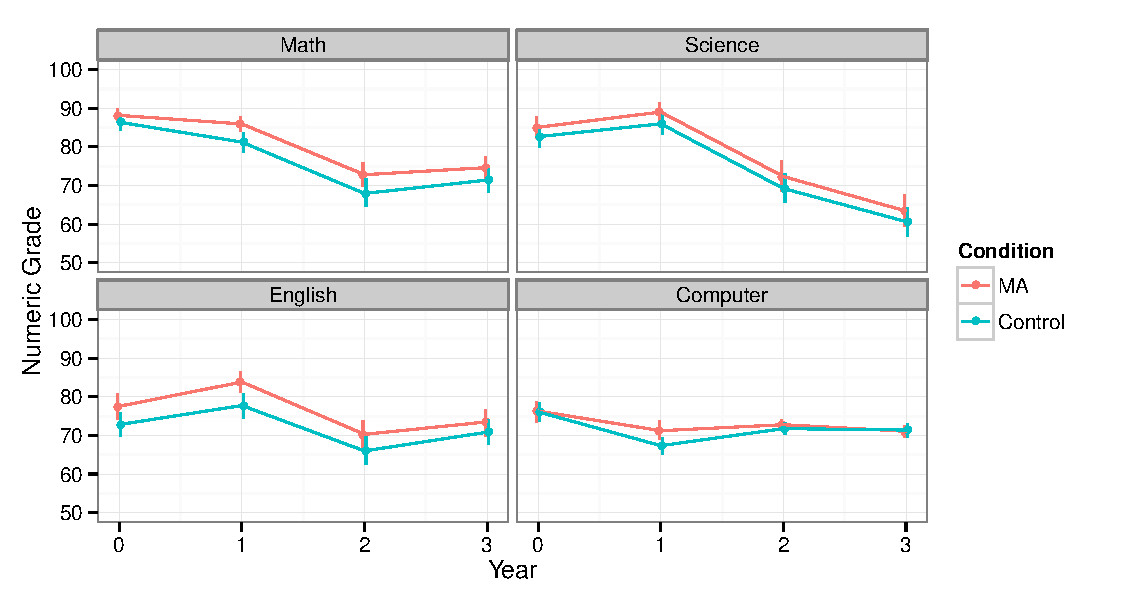
\includegraphics[width=6.5in]{figures/grades.pdf}
\end{center}
\caption{Academic outcome measures for the two intervention conditions, plotted by study year. Error bars show 95\% confidence intervals computed by non-parametric bootstrap.}
\label{fig:grades}
\end{figure}

Due to limited grade variance in Music, Art, and Physical Education, we only analyzed data from Math, English, Science, and Computer. Means are shown in Figure~\ref{fig:grades}. 

There was an overall trend in our dataset to see higher grades for the MA group, but this trend is confounded with assignment to class, since the majority of MA students were grouped together in a single class. Also, the grading criteria for each class varied by year, making it difficult to assess growth. For example, science grades declined over time, even though students' total science knowledge almost certainly increased over that time period. In addition, classroom teachers were not blind to the assignment of students to condition. Thus, academic outcome measures may be subject to bias and should be interpreted with caution. 

We observed no reliable year by condition interactions in the longitudinal models, though we did see some trends toward an interaction in some models of math grades independent growth model, $p = .06$) and computer class grades (quadratic and independent growth models, $p = .07$). 
 
% \subsection{Additional Analysis of Abacus-Only Tasks}

% \begin{figure}[H]
% \begin{center}
% 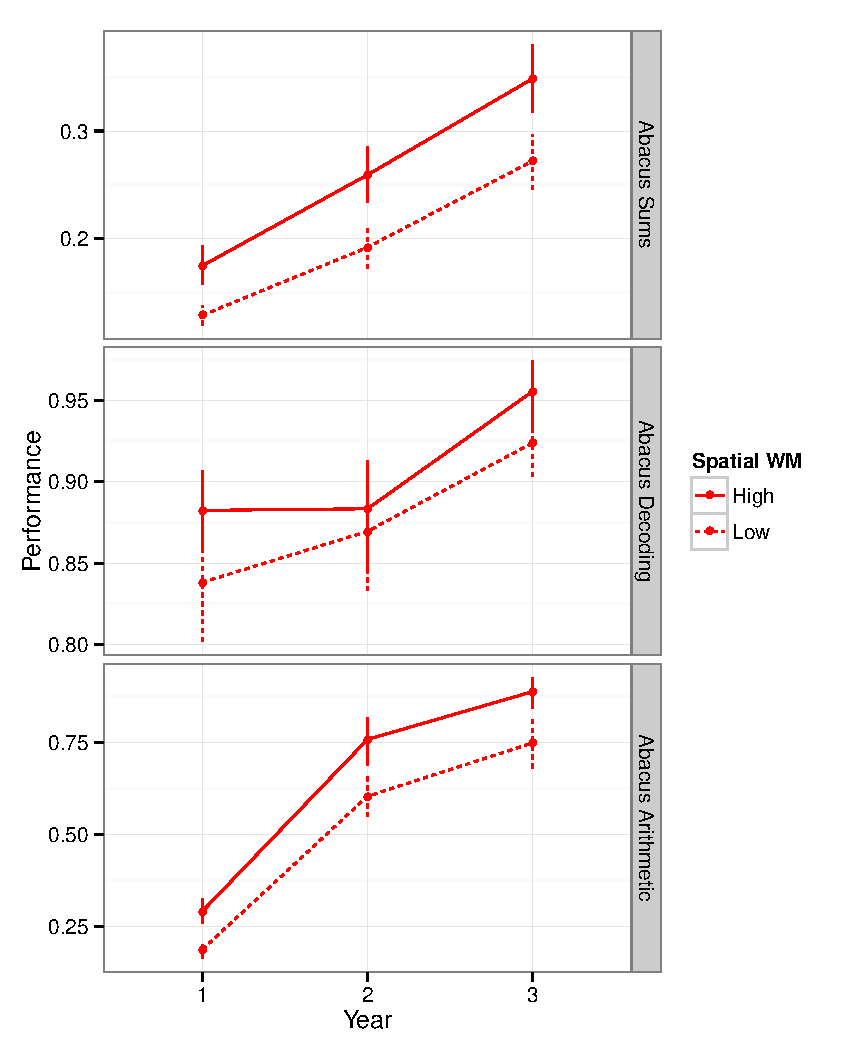
\includegraphics[width=4.5in]{figures/abacus_by_swm.pdf}
% \end{center}
% \caption{Performance on the Abacus Only Sums, Decoding, and Arithmetic tasks (administered in years 1 -- 3), plotted by a median split on spatial working memory. Error bars show 95\% confidence intervals computed by non-parametric bootstrap.}
% \label{fig:abacusonly}
% \end{figure}

% Performance on the Abacus Only tasks is shown in Figure \ref{fig:abacusonly}. Performance is split by spatial working memory span during Year 0. All three measures showed significant main effects of spatial working memory (see Main Text).

\subsection{Additional Mediation Analysis}

We show two additional mediation analyses described in the main text. The first is the effect of spatial working memory as a mediator of performance on the WJ-III arithmetic task (Figure~\ref{fig:wj3swm}). Children in the MA condition who performed above the median on the spatial working memory task in Year 0 subsequently showed stronger growth in their WJ-III performance. 


\begin{figure}[H]
\begin{center}
\includegraphics[width=4.5in]{figures/wj_by_swm.pdf}
\end{center}
\caption{WJ-III arithmetic performance split by condition and median performance on the spatial working memory measure, plotted by study year. Error bars show 95\% confidence intervals computed by non-parametric bootstrap.}
\label{fig:wj3swm}
\end{figure}

The second effect is that of approximate number acuity (Weber fraction, as measured by the number comparison task) on WJ-III performance. This effect is shown in Figure \ref{fig:wj3ans}. Those children in the control group with higher than median Weber fractions in Year 0 subsequently showed worse performance on the WJ-III (recall that lower Weber fractions indicate better acuity). 

\begin{figure}[H]
\begin{center}
\includegraphics[width=4.5in]{figures/wj_by_ans.pdf}
\end{center}
\caption{WJ-III arithmetic performance split by condition and median performance on the Number Comparison measure, plotted by study year. Note that a larger Weber fraction indicates lower numerical acuity. Error bars show 95\% confidence intervals computed by non-parametric bootstrap.}
\label{fig:wj3ans}
\end{figure}

In addition, we show the effect of splitting by verbal working memory on arithmetic in Figure \ref{fig:arithvwm}. Although there are substantial differences in arithmetic performance predicted by Year 0 verbal working memory, there is no interaction with intervention condition (compare to Figure 4 in the main text). This result is borne out by both the linear and quadratic growth models, which show no interaction of intervention condition and verbal working memory ($p$s $> .52$).

\begin{figure}[H]
\begin{center}
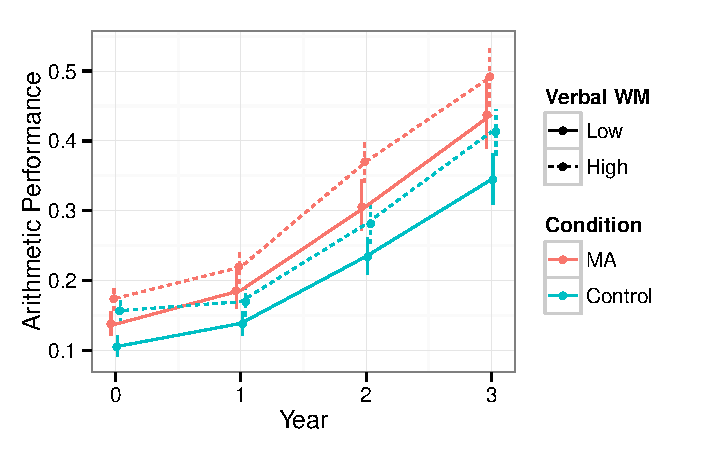
\includegraphics[width=4.5in]{figures/arith_by_vwm.pdf}
\end{center}
\caption{Arithmetic performance split by condition and median performance on verbal working memory, plotted by study year. Error bars show 95\% confidence intervals computed by non-parametric bootstrap.}
\label{fig:arithvwm}
\end{figure}

\subsection{Additional Analysis of Spatial Working Memory Data}

In this section, we describe analyses addressing whether we saw a ceiling effect in our spatial working memory task; had there been such a ceiling effect, we might have been unable to detect transfer effects. Figure \ref{fig:densities} shows the distributions of spatial working memory scores; there is no visual suggestion of right-censoring of these distributions. 

\begin{figure}[H]
\begin{center}
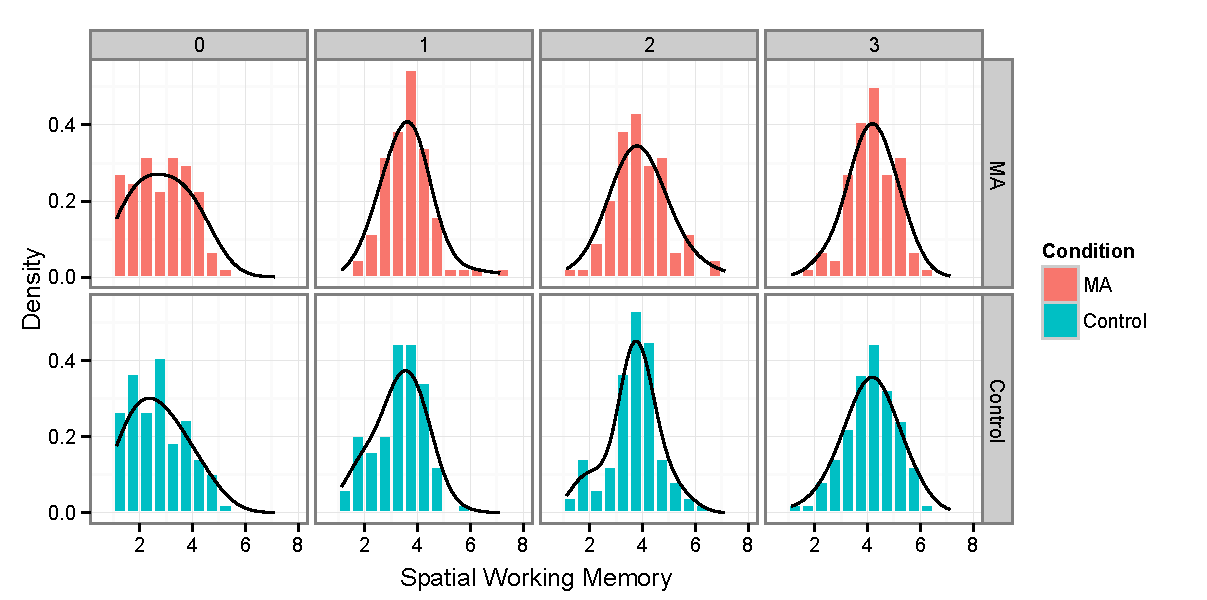
\includegraphics[width=6.5in]{figures/swmdensities.pdf}
\end{center}
\caption{The distribution of spatial working memory scores across intervention groups and years. Histograms show the empirical probabilities, while lines show a smoothed density estimate.}
\label{fig:densities}
\end{figure}

A second analysis suggest that the range of spatial working memory scores we observed was low (congruent with the low socioeconomic status of our participants) but that we nevertheless saw substantial development with age as well as some quite high (adult-level) performances. As part of separate studies, we administered the same spatial working memory task to two other groups: a group of high socioeconomic status children tested at a mental abacus after-school program in the same city as our intervention site (N=67), and a group of college-age adults in the United States (N=20). 

Data from all three groups are shown in Figure \ref{fig:swm}. Clearly, there is no ceiling effect in the Intervention group Spatial Working Memory data. Mean scores for both other groups are substantially higher than those for the current study, and there are strong indications of developmental trends in both groups of children, suggesting that the children in our study would be likely to improve substantially on this measure. 

\begin{figure}[H]
\begin{center}
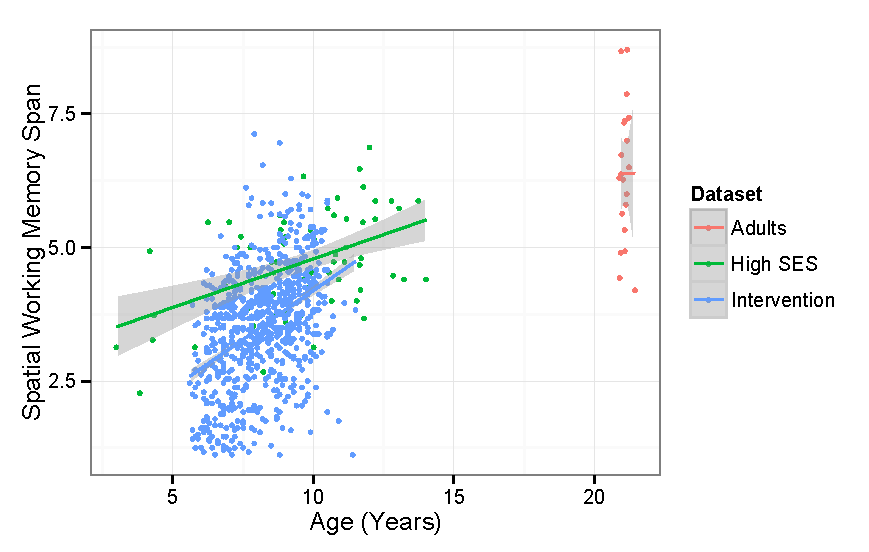
\includegraphics[width=4.5in]{figures/swm.pdf}
\end{center}
\caption{Spatial working memory scores plotted by age for three populations. Each point represents an individual participant. Lines show best fitting linear regression with 95\% confidence intervals. Adult data are plotted at age 21, as individual ages were not available.}
\label{fig:swm}
\end{figure}


\subsection{Additional Analysis of Classroom Effects}

As described above, there were three classrooms that participated in our intervention. In the first classroom (labeled A for convenience), all students received MA instruction. In a second class (B), students were split between MA and control instruction. In the third class (C), all students received control instruction. Four students are excluded for this analysis due to having changed classes or uncertainty about which classroom they had been placed into during one or more years of the study. In Figures \ref{fig:mathclass1} -- \ref{fig:cogclass2} we show math and cognitive measures replotted by class and intervention group. Qualitatively, it appears that control students in class B (who had MA students in their classroom) showed some benefits on several of the measures, especially arithmetic and WJ-III. 


\begin{figure}[H]
\begin{center}
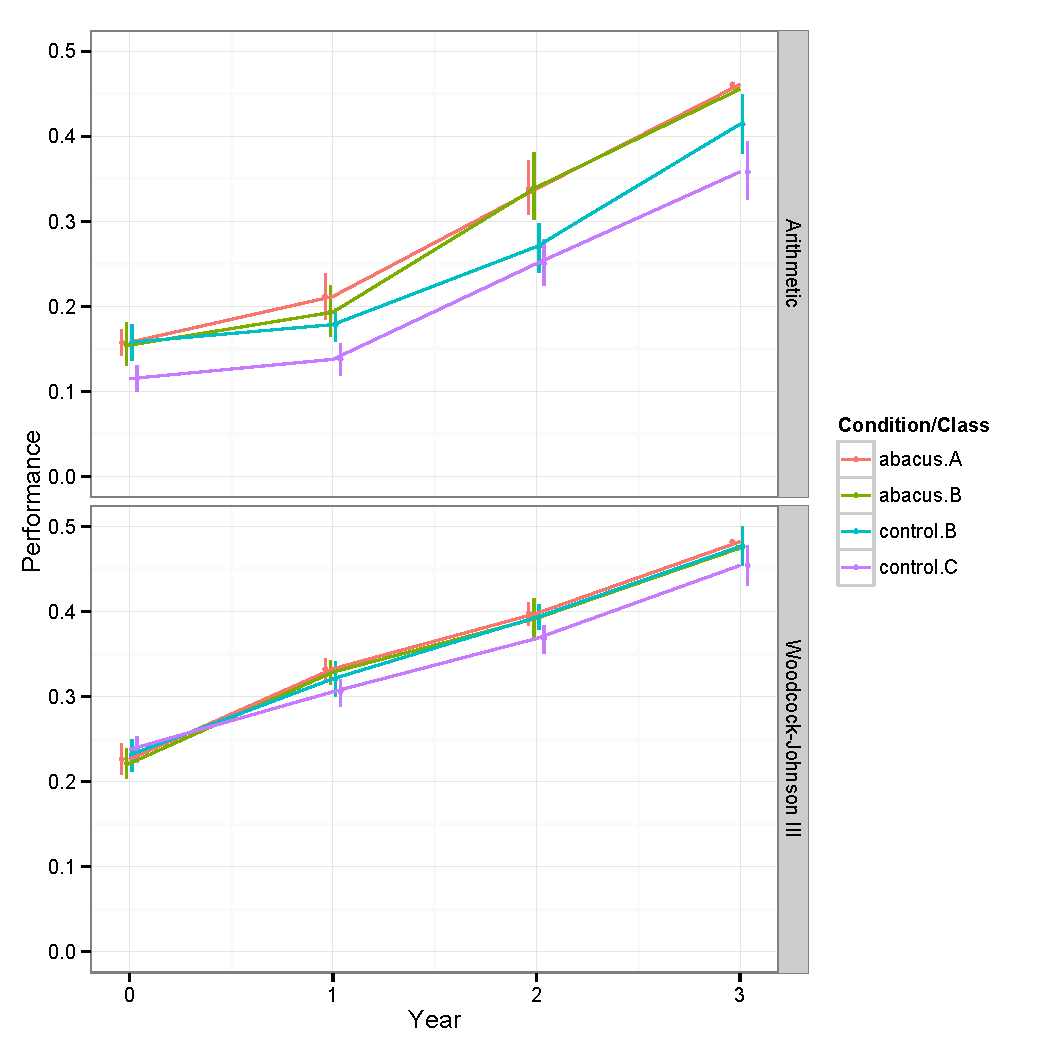
\includegraphics[width=5.5in]{figures/math1_class.pdf}
\end{center}
\caption{Performance on arithmetic and WJ-III, split by intervention group and class. Class A received MA instruction; Class B was split between MA and control; Class C received control instruction. Error bars show 95\% confidence intervals computed by non-parametric bootstrap.}
\label{fig:mathclass1}
\end{figure}

\begin{figure}[H]
\begin{center}
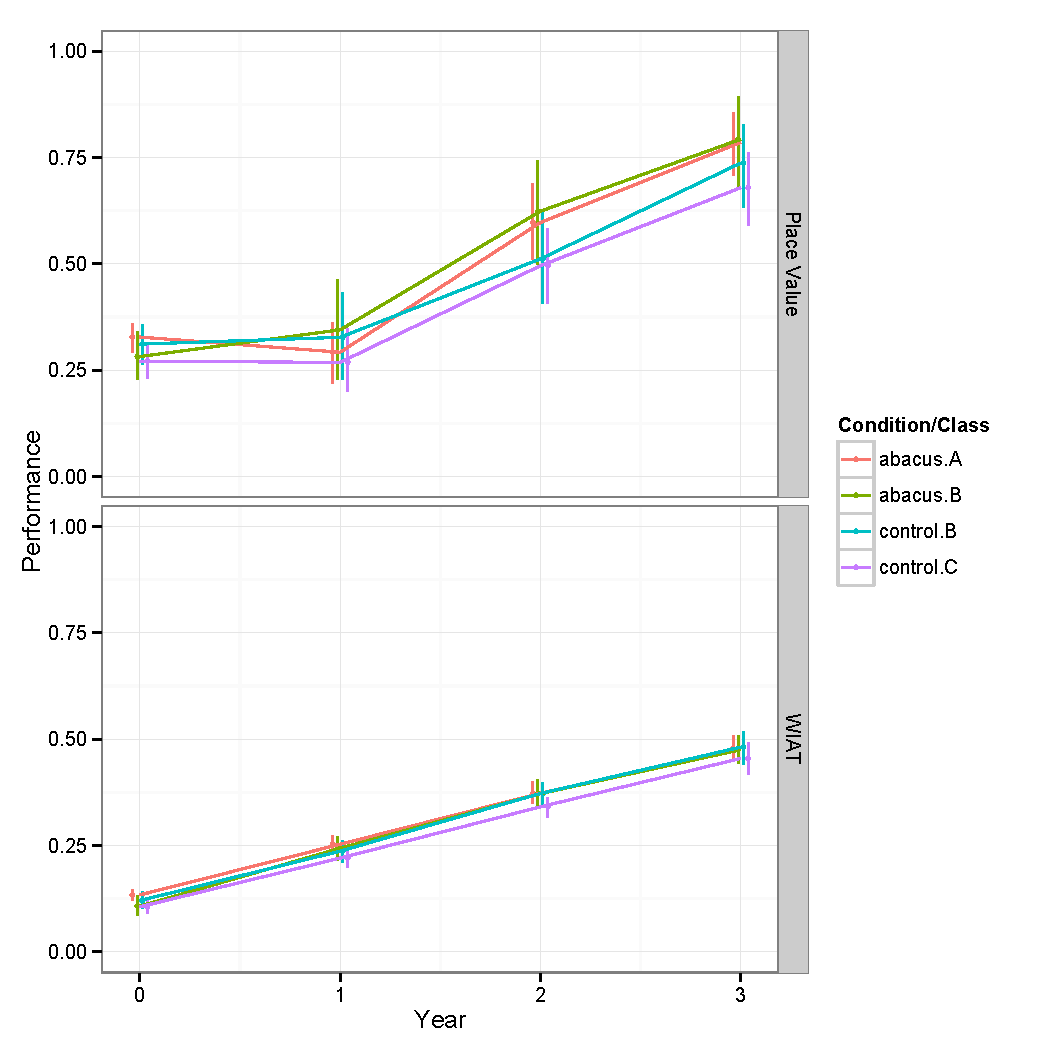
\includegraphics[width=5.5in]{figures/math2_class.pdf}
\end{center}
\caption{Performance on Place Value and WIAT, split by intervention group and class. Class A received MA instruction; Class B was split between MA and control; Class C received control instruction. Error bars show 95\% confidence intervals computed by non-parametric bootstrap.}
\label{fig:mathclass2}
\end{figure}


\begin{figure}[H]
\begin{center}
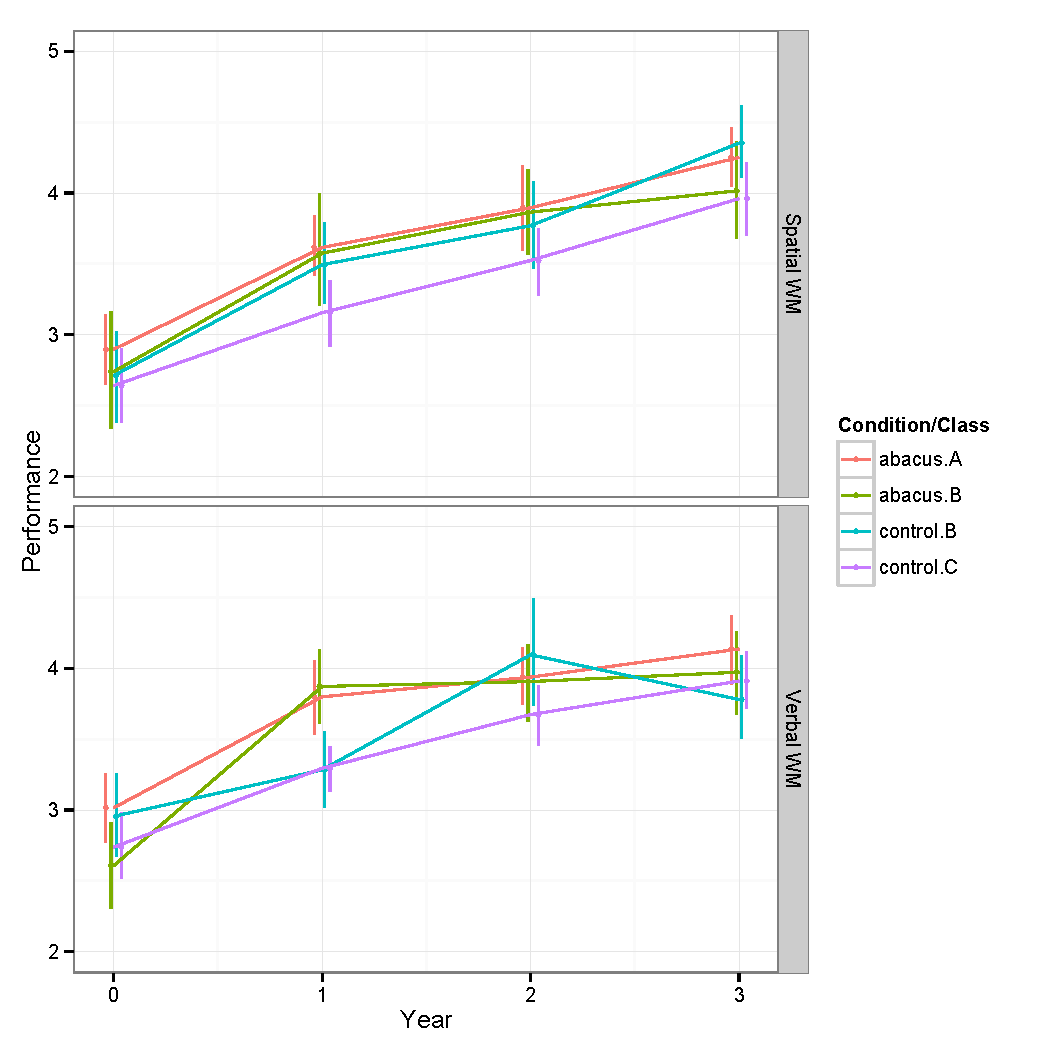
\includegraphics[width=5.5in]{figures/cog1_class.pdf}
\end{center}
\caption{Performance on spatial and verbal working memory, split by intervention group and class. Class A received MA instruction; Class B was split between MA and control; Class C received control instruction. Error bars show 95\% confidence intervals computed by non-parametric bootstrap.}
\label{fig:cogclass1}
\end{figure}


\begin{figure}[H]
\begin{center}
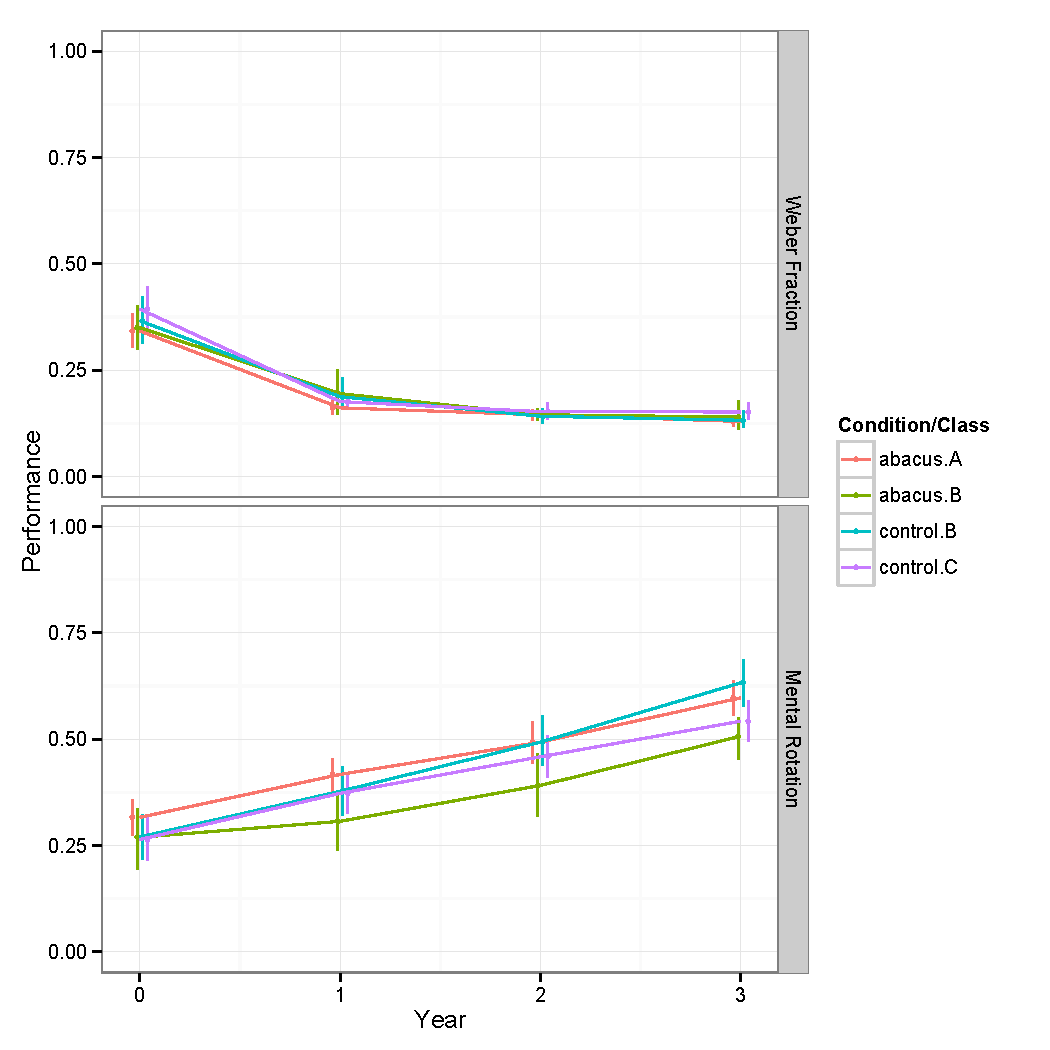
\includegraphics[width=5.5in]{figures/cog2_class.pdf}
\end{center}
\caption{Performance on ANS and mental rotation, split by intervention group and class. Class A received MA instruction; Class B was split between MA and control; Class C received control instruction. Error bars show 95\% confidence intervals computed by non-parametric bootstrap.}
\label{fig:cogclass2}
\end{figure}

To quantify these trends, we used the same longitudinal growth models described above; for simplicity we examine the linear and quadratic models only. We defined a model that included interactions between year, intervention condition, and classroom, and conducted likelihood ratio tests against a model that only included main effects of classroom (to control for general baseline differences between classes). No classroom effects reached significance in the linear or quadratic growth models. 

In an additional analysis, we examined whether classroom assignment affected uptake of the abacus intervention. Results of this analysis are plotted in Figure \ref{fig:abacus_class}. The only measure in which there was a hint of a difference was in the Abacus Decoding task, and no longitudinal model reached significance for any year-by-class interactions (all $p$s $> .17$). 

\begin{figure}[H]
\begin{center}
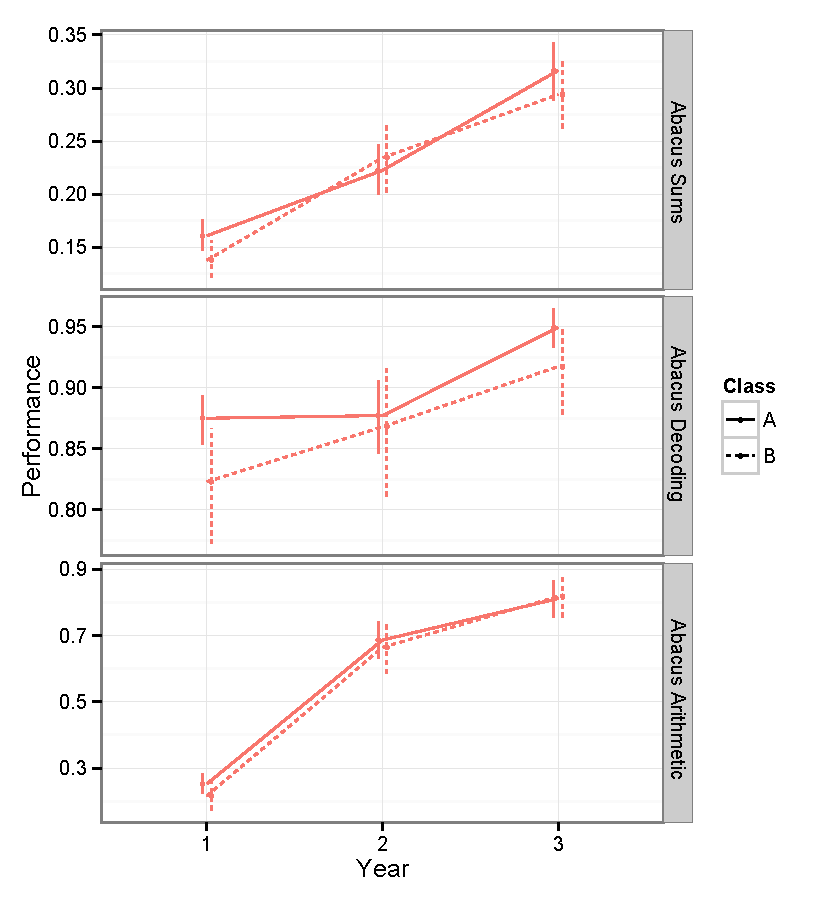
\includegraphics[width=4.5in]{figures/abacus_class.pdf}
\end{center}
\caption{Performance on the Abacus Only Sums, Decoding, and Arithmetic tasks (across years 1 -- 3), plotted by class. Class A received MA instruction; Class B was split between MA and control (only MA participants are plotted). Error bars show 95\% confidence intervals computed by non-parametric bootstrap.}
\label{fig:abacus_class}
\end{figure}


In sum: Control children in the mixed MA/control classroom showed numerically-increased performance on some math measures. Since these students were sharing regular math instruction with a group of MA children, this effect might be driven by the presence of MA children leading to spillover effects in classroom instruction (whether because the overall level of instruction was higher or due to other mechanisms of peer influence).

\subsection{Task Variability}

We speculate that one reason our arithmetic measure might have shown larger intervention effects is because it is a more sensitive measure that better taps differences between students in arithmetic. The standardized tests---the WJ-III especially---feature relatively few items that probe content learned in early grade school. Thus, they may be less able to capture variability among young children than our own task by virtue of how they are designed. For example, considering 1- to 3-digit addition problems involving positive numbers, the WIAT has 8 and WJ has 6. For subtraction problems, the WIAT has 8 and the WJ has 6. Fully 1/3 of WJ questions involve knowledge of algebra, exponents, trigonometry, and other advanced material. The WIAT, while less advanced, still has several questions concerning, e.g., adding fractions with mixed denominators. 

\begin{figure}[H]
\begin{center}
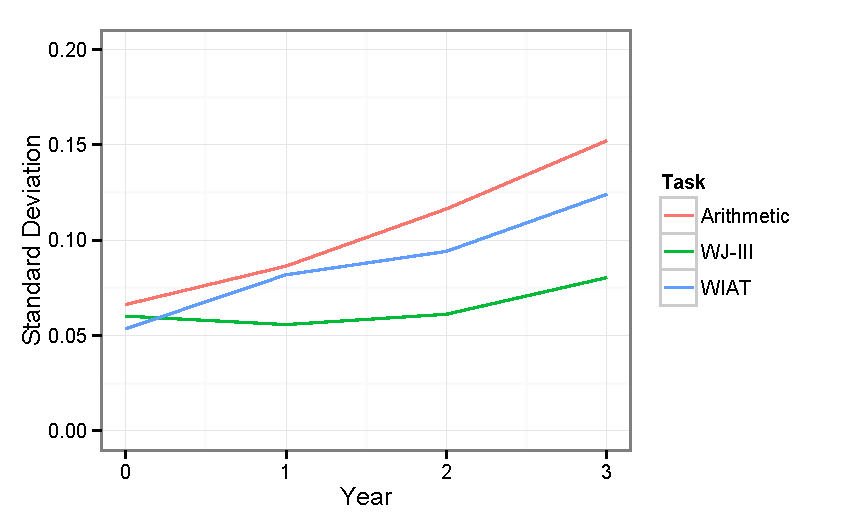
\includegraphics[width=4.5in]{figures/SDs.pdf}
\end{center}
\caption{Standard deviations for the three arithmetic measures, plotted by year. Each measure was normalized into the range 0--1.}
\label{fig:sds}
\end{figure}

Two pieces of evidence provide partial support for this intuition. First, we show in Figure \ref{fig:sds} an analysis of the standard deviation of participants' performance on each of the three math measures that include arithmetic problems (Arithmetic, WIAT, and WJ-III). All scores were in the 0 -- 1 interval.  On this measure, the WJ-III shows less variability than the other two measures. A second piece of evidence comes from the year-to-year correlations between students' performance. Across the three measures, the arithmetic measure had the highest average year-to-year correlation across all pairs of measurements ($r = .56$, compared with .47 and .50 for the WJ-III and WIAT, respectively). 

\subsection{Randomization Analysis and Propensity Score Matching}

As noted in the main text, despite randomization of students to classrooms, we nevertheless observed some differences between groups at initiation of the study. Pairwise tests on all measures are given in Table \ref{tab:pairwise}. We note that these $p$ values are uncorrected for multiple comparisons; using a standard Bonferroni correction, none would be considered significant at the .05 level. 

% latex table generated in R 3.1.2 by xtable 1.7-4 package
% Sun Jun 28 19:02:07 2015
\begin{table}[ht]
\centering
\caption{\label{tab:pairwise} Pairwise $t$-tests of Year 0 performance across tasks).}
\begin{tabular}{lrrrr}
  \hline
measure & $M_{MA}$ & $M_{Control}$ & $t$ & $p$ \\ 
  \hline
WIAT & 0.16 & 0.14 & 2.08 & 0.04 \\ 
WJ-III & 0.23 & 0.24 & -1.21 & 0.23 \\ 
Arithmetic & 0.16 & 0.13 & 2.65 & 0.01 \\ 
Place Value & 0.31 & 0.29 & 0.93 & 0.36 \\ 
Raven's & 0.56 & 0.49 & 2.10 & 0.04 \\ 
ANS & 0.35 & 0.38 & -1.36 & 0.18 \\ 
Spatial WM & 2.83 & 2.68 & 0.98 & 0.33 \\ 
Verbal WM & 2.89 & 2.82 & 0.51 & 0.61 \\ 
Mental Rotation & 0.30 & 0.27 & 1.23 & 0.22 \\ 
   \hline
\end{tabular}
\end{table}

For this reason, we pursued a statistical approach to equate the groups for further analysis, known as propensity score matching \cite{rosenbaum1983,sekhon2008}. This technique is commonly used for observational studies rather than intervention studies like ours, but can also be applied as a method for controlling differences between groups. In brief, propensity score matching is performed via two steps. First, using logistic regression, a ``propensity score'' is constructed. This score estimates the probability that participants will find themselves in one group or the other, on the basis of predictor variables (in our case, mathematical ability factors, e.g. arithmetic, WIAT, WJ-III, and place value scores). Second, an artificial control group for the study is resampled with replacement from the real control group so as to equate the propensity score for both groups. Once this pseudo-control group is constructed, the original statistical analyses can be done comparing them to the intervention group. 

In practice, we used the \texttt{Matching} package for R \cite{sekhon2008} to construct 1000 propensity-matched control groups with replacement and random tie-breaking, using the propensity score variables above. Results did not differ substantially if we used subsets of these propensity score variables. We then ran our same longitudinal model comparison analyses (using linear growth models) on each resampled control group. 

The propensity score matching approach yielded consistently significant intervention by time results for the arithmetic measure ($p_{avg} = .002$) but failed to yield significant results for the other math measures (all $p$s $>.33$). $t$-tests of Year 3 performance on these propensity-matched groups yielded the same basic result. We interpret these findings with caution, however, as using propensity score matching \emph{after} randomization is a very conservative procedure. In practice, ``unhappy'' randomization can certainly occur but given the number of comparisons in Table \ref{tab:pairwise}, we may be over-correcting and reducing statistical power by inflating the mathematics competence of our artificial control groups. 

\newpage
\bibliographystyle{apacite}
\bibliography{sibib}
 
\end{document}


% \subsection{Longitudinal Model Results}

% \subsection{Linear Growth Models}

% % latex table generated in R 3.0.2 by xtable 1.7-1 package
% % Fri Dec 27 13:04:53 2013
% \begin{table}[H]
% \centering
% \begin{tabular}{rrrr}
%   \hline
%  & Estimate & Std. Error & t value \\ 
%   \hline
% (Intercept) & 0.13 & 0.01 & 21.59 \\ 
%   year & 0.12 & 0.00 & 42.79 \\ 
%   conditioncontrol & -0.02 & 0.01 & -2.47 \\ 
%    \hline
% \end{tabular}
% \caption{Linear mixed effects model coefficients for a linear growth model with no year * condition interaction term for WIAT.} 
% \end{table}

% % latex table generated in R 3.0.2 by xtable 1.7-1 package
% % Fri Dec 27 13:04:53 2013
% \begin{table}[H]
% \centering
% \begin{tabular}{rrrr}
%   \hline
%  & Estimate & Std. Error & t value \\ 
%   \hline
% (Intercept) & 0.13 & 0.01 & 21.33 \\ 
%   year & 0.12 & 0.00 & 29.29 \\ 
%   conditioncontrol & -0.02 & 0.01 & -2.43 \\ 
%   year:conditioncontrol & 0.00 & 0.01 & 0.09 \\ 
%    \hline
% \end{tabular}
% \caption{Linear mixed effects model coefficients for a linear growth model with year * condition interaction term for WIAT.} 
% \end{table}

% % latex table generated in R 3.0.2 by xtable 1.7-1 package
% % Fri Dec 27 13:04:53 2013
% \begin{table}[H]
% \centering
% \begin{tabular}{lrrrrrrrr}
%   \hline
%  & Df & AIC & BIC & logLik & deviance & Chisq & Chi Df & Pr($>$Chisq) \\ 
%   \hline
% m2 & 7 & -1696.02 & -1663.95 & 855.01 & -1710.02 &  &  &  \\ 
%   m1 & 8 & -1694.03 & -1657.38 & 855.02 & -1710.03 & 0.01 & 1 & 0.9277 \\ 
%    \hline
% \end{tabular}
% \caption{Likelihood comparison for the preceding linear models.} 
% \end{table}

% % latex table generated in R 3.0.2 by xtable 1.7-1 package
% % Fri Dec 27 13:04:53 2013
% \begin{table}[H]
% \centering
% \begin{tabular}{rrrr}
%   \hline
%  & Estimate & Std. Error & t value \\ 
%   \hline
% (Intercept) & 0.24 & 0.01 & 46.46 \\ 
%   year & 0.08 & 0.00 & 43.85 \\ 
%   conditioncontrol & -0.00 & 0.01 & -0.69 \\ 
%    \hline
% \end{tabular}
% \caption{Linear mixed effects model coefficients for a linear growth model with no year * condition interaction term for WJ-III.} 
% \end{table}

% % latex table generated in R 3.0.2 by xtable 1.7-1 package
% % Fri Dec 27 13:04:53 2013
% \begin{table}[H]
% \centering
% \begin{tabular}{rrrr}
%   \hline
%  & Estimate & Std. Error & t value \\ 
%   \hline
% (Intercept) & 0.23 & 0.01 & 44.40 \\ 
%   year & 0.08 & 0.00 & 32.43 \\ 
%   conditioncontrol & 0.00 & 0.01 & 0.23 \\ 
%   year:conditioncontrol & -0.01 & 0.00 & -2.52 \\ 
%    \hline
% \end{tabular}
% \caption{Linear mixed effects model coefficients for a linear growth model with year * condition interaction term for WJ-III.} 
% \end{table}

% % latex table generated in R 3.0.2 by xtable 1.7-1 package
% % Fri Dec 27 13:04:53 2013
% \begin{table}[H]
% \centering
% \begin{tabular}{lrrrrrrrr}
%   \hline
%  & Df & AIC & BIC & logLik & deviance & Chisq & Chi Df & Pr($>$Chisq) \\ 
%   \hline
% m2 & 7 & -2169.36 & -2137.08 & 1091.68 & -2183.36 &  &  &  \\ 
%   m1 & 8 & -2173.69 & -2136.81 & 1094.85 & -2189.69 & 6.33 & 1 & 0.0118 \\ 
%    \hline
% \end{tabular}
% \caption{Likelihood comparison for the preceding linear models.} 
% \end{table}

% % latex table generated in R 3.0.2 by xtable 1.7-1 package
% % Fri Dec 27 13:04:53 2013
% \begin{table}[H]
% \centering
% \begin{tabular}{rrrr}
%   \hline
%  & Estimate & Std. Error & t value \\ 
%   \hline
% (Intercept) & 0.13 & 0.01 & 20.06 \\ 
%   year & 0.09 & 0.00 & 28.69 \\ 
%   conditioncontrol & -0.03 & 0.01 & -3.68 \\ 
%    \hline
% \end{tabular}
% \caption{Linear mixed effects model coefficients for a linear growth model with no year * condition interaction term for Arithmetic Task.} 
% \end{table}

% % latex table generated in R 3.0.2 by xtable 1.7-1 package
% % Fri Dec 27 13:04:53 2013
% \begin{table}[H]
% \centering
% \begin{tabular}{rrrr}
%   \hline
%  & Estimate & Std. Error & t value \\ 
%   \hline
% (Intercept) & 0.13 & 0.01 & 19.46 \\ 
%   year & 0.11 & 0.00 & 22.61 \\ 
%   conditioncontrol & -0.03 & 0.01 & -3.09 \\ 
%   year:conditioncontrol & -0.02 & 0.01 & -3.33 \\ 
%    \hline
% \end{tabular}
% \caption{Linear mixed effects model coefficients for a linear growth model with year * condition interaction term for Arithmetic Task.} 
% \end{table}

% % latex table generated in R 3.0.2 by xtable 1.7-1 package
% % Fri Dec 27 13:04:53 2013
% \begin{table}[H]
% \centering
% \begin{tabular}{lrrrrrrrr}
%   \hline
%  & Df & AIC & BIC & logLik & deviance & Chisq & Chi Df & Pr($>$Chisq) \\ 
%   \hline
% m2 & 7 & -1500.62 & -1468.37 & 757.31 & -1514.62 &  &  &  \\ 
%   m1 & 8 & -1509.54 & -1472.68 & 762.77 & -1525.54 & 10.92 & 1 & 0.0010 \\ 
%    \hline
% \end{tabular}
% \caption{Likelihood comparison for the preceding linear models.} 
% \end{table}

% % latex table generated in R 3.0.2 by xtable 1.7-1 package
% % Fri Dec 27 13:04:54 2013
% \begin{table}[H]
% \centering
% \begin{tabular}{rrrr}
%   \hline
%  & Estimate & Std. Error & t value \\ 
%   \hline
% (Intercept) & 0.25 & 0.02 & 12.06 \\ 
%   year & 0.16 & 0.01 & 18.59 \\ 
%   conditioncontrol & -0.03 & 0.03 & -1.10 \\ 
%    \hline
% \end{tabular}
% \caption{Linear mixed effects model coefficients for a linear growth model with no year * condition interaction term for Place Value Task.} 
% \end{table}

% % latex table generated in R 3.0.2 by xtable 1.7-1 package
% % Fri Dec 27 13:04:54 2013
% \begin{table}[H]
% \centering
% \begin{tabular}{rrrr}
%   \hline
%  & Estimate & Std. Error & t value \\ 
%   \hline
% (Intercept) & 0.24 & 0.02 & 11.33 \\ 
%   year & 0.18 & 0.01 & 14.00 \\ 
%   conditioncontrol & -0.01 & 0.03 & -0.51 \\ 
%   year:conditioncontrol & -0.03 & 0.02 & -1.62 \\ 
%    \hline
% \end{tabular}
% \caption{Linear mixed effects model coefficients for a linear growth model with year * condition interaction term for Place Value Task.} 
% \end{table}

% % latex table generated in R 3.0.2 by xtable 1.7-1 package
% % Fri Dec 27 13:04:54 2013
% \begin{table}[H]
% \centering
% \begin{tabular}{lrrrrrrrr}
%   \hline
%  & Df & AIC & BIC & logLik & deviance & Chisq & Chi Df & Pr($>$Chisq) \\ 
%   \hline
% m2 & 7 & 112.68 & 144.98 & -49.34 & 98.68 &  &  &  \\ 
%   m1 & 8 & 112.06 & 148.97 & -48.03 & 96.06 & 2.62 & 1 & 0.1057 \\ 
%    \hline
% \end{tabular}
% \caption{Likelihood comparison for the preceding linear models.} 
% \end{table}

% % latex table generated in R 3.0.2 by xtable 1.7-1 package
% % Fri Dec 27 13:04:54 2013
% \begin{table}[H]
% \centering
% \begin{tabular}{rrrr}
%   \hline
%  & Estimate & Std. Error & t value \\ 
%   \hline
% (Intercept) & 0.54 & 0.02 & 28.20 \\ 
%   year & 0.01 & 0.01 & 1.06 \\ 
%   conditioncontrol & -0.00 & 0.02 & -0.08 \\ 
%    \hline
% \end{tabular}
% \caption{Linear mixed effects model coefficients for a linear growth model with no year * condition interaction term for Raven's Progressive Matrices.} 
% \end{table}

% % latex table generated in R 3.0.2 by xtable 1.7-1 package
% % Fri Dec 27 13:04:54 2013
% \begin{table}[H]
% \centering
% \begin{tabular}{rrrr}
%   \hline
%  & Estimate & Std. Error & t value \\ 
%   \hline
% (Intercept) & 0.56 & 0.02 & 25.95 \\ 
%   year & -0.01 & 0.01 & -0.73 \\ 
%   conditioncontrol & -0.04 & 0.03 & -1.35 \\ 
%   year:conditioncontrol & 0.02 & 0.01 & 2.00 \\ 
%    \hline
% \end{tabular}
% \caption{Linear mixed effects model coefficients for a linear growth model with year * condition interaction term for Raven's Progressive Matrices.} 
% \end{table}

% % latex table generated in R 3.0.2 by xtable 1.7-1 package
% % Fri Dec 27 13:04:54 2013
% \begin{table}[H]
% \centering
% \begin{tabular}{lrrrrrrrr}
%   \hline
%  & Df & AIC & BIC & logLik & deviance & Chisq & Chi Df & Pr($>$Chisq) \\ 
%   \hline
% m2 & 7 & -325.77 & -293.61 & 169.89 & -339.77 &  &  &  \\ 
%   m1 & 8 & -327.76 & -291.01 & 171.88 & -343.76 & 3.99 & 1 & 0.0457 \\ 
%    \hline
% \end{tabular}
% \caption{Likelihood comparison for the preceding linear models.} 
% \end{table}

% % latex table generated in R 3.0.2 by xtable 1.7-1 package
% % Fri Dec 27 13:04:54 2013
% \begin{table}[H]
% \centering
% \begin{tabular}{rrrr}
%   \hline
%  & Estimate & Std. Error & t value \\ 
%   \hline
% (Intercept) & 0.30 & 0.01 & 29.01 \\ 
%   year & -0.07 & 0.00 & -17.52 \\ 
%   conditioncontrol & 0.01 & 0.01 & 0.94 \\ 
%    \hline
% \end{tabular}
% \caption{Linear mixed effects model coefficients for a linear growth model with no year * condition interaction term for Number Comparison.} 
% \end{table}

% % latex table generated in R 3.0.2 by xtable 1.7-1 package
% % Fri Dec 27 13:04:54 2013
% \begin{table}[H]
% \centering
% \begin{tabular}{rrrr}
%   \hline
%  & Estimate & Std. Error & t value \\ 
%   \hline
% (Intercept) & 0.30 & 0.01 & 22.58 \\ 
%   year & -0.07 & 0.01 & -12.01 \\ 
%   conditioncontrol & 0.01 & 0.02 & 0.68 \\ 
%   year:conditioncontrol & -0.00 & 0.01 & -0.24 \\ 
%    \hline
% \end{tabular}
% \caption{Linear mixed effects model coefficients for a linear growth model with year * condition interaction term for Number Comparison.} 
% \end{table}

% % latex table generated in R 3.0.2 by xtable 1.7-1 package
% % Fri Dec 27 13:04:54 2013
% \begin{table}[H]
% \centering
% \begin{tabular}{lrrrrrrrr}
%   \hline
%  & Df & AIC & BIC & logLik & deviance & Chisq & Chi Df & Pr($>$Chisq) \\ 
%   \hline
% m2 & 7 & -1147.74 & -1115.75 & 580.87 & -1161.74 &  &  &  \\ 
%   m1 & 8 & -1145.80 & -1109.24 & 580.90 & -1161.80 & 0.06 & 1 & 0.8056 \\ 
%    \hline
% \end{tabular}
% \caption{Likelihood comparison for the preceding linear models.} 
% \end{table}

% % latex table generated in R 3.0.2 by xtable 1.7-1 package
% % Fri Dec 27 13:04:55 2013
% \begin{table}[H]
% \centering
% \begin{tabular}{rrrr}
%   \hline
%  & Estimate & Std. Error & t value \\ 
%   \hline
% (Intercept) & 2.94 & 0.08 & 35.51 \\ 
%   year & 0.45 & 0.03 & 16.18 \\ 
%   conditioncontrol & -0.19 & 0.09 & -2.02 \\ 
%    \hline
% \end{tabular}
% \caption{Linear mixed effects model coefficients for a linear growth model with no year * condition interaction term for spatial working memory.} 
% \end{table}

% % latex table generated in R 3.0.2 by xtable 1.7-1 package
% % Fri Dec 27 13:04:55 2013
% \begin{table}[H]
% \centering
% \begin{tabular}{rrrr}
%   \hline
%  & Estimate & Std. Error & t value \\ 
%   \hline
% (Intercept) & 2.98 & 0.10 & 30.75 \\ 
%   year & 0.43 & 0.04 & 10.62 \\ 
%   conditioncontrol & -0.25 & 0.13 & -1.90 \\ 
%   year:conditioncontrol & 0.04 & 0.06 & 0.68 \\ 
%    \hline
% \end{tabular}
% \caption{Linear mixed effects model coefficients for a linear growth model with year * condition interaction term for spatial working memory.} 
% \end{table}

% % latex table generated in R 3.0.2 by xtable 1.7-1 package
% % Fri Dec 27 13:04:55 2013
% \begin{table}[H]
% \centering
% \begin{tabular}{lrrrrrrrr}
%   \hline
%  & Df & AIC & BIC & logLik & deviance & Chisq & Chi Df & Pr($>$Chisq) \\ 
%   \hline
% m2 & 7 & 2021.78 & 2054.08 & -1003.89 & 2007.78 &  &  &  \\ 
%   m1 & 8 & 2023.32 & 2060.24 & -1003.66 & 2007.32 & 0.46 & 1 & 0.4975 \\ 
%    \hline
% \end{tabular}
% \caption{Likelihood comparison for the preceding linear models.} 
% \end{table}

% % latex table generated in R 3.0.2 by xtable 1.7-1 package
% % Fri Dec 27 13:04:55 2013
% \begin{table}[H]
% \centering
% \begin{tabular}{rrrr}
%   \hline
%  & Estimate & Std. Error & t value \\ 
%   \hline
% (Intercept) & 3.14 & 0.08 & 41.67 \\ 
%   year & 0.37 & 0.03 & 14.13 \\ 
%   conditioncontrol & -0.24 & 0.09 & -2.79 \\ 
%    \hline
% \end{tabular}
% \caption{Linear mixed effects model coefficients for a linear growth model with no year * condition interaction term for Verbal Working Memory.} 
% \end{table}

% % latex table generated in R 3.0.2 by xtable 1.7-1 package
% % Fri Dec 27 13:04:55 2013
% \begin{table}[H]
% \centering
% \begin{tabular}{rrrr}
%   \hline
%  & Estimate & Std. Error & t value \\ 
%   \hline
% (Intercept) & 3.13 & 0.09 & 35.72 \\ 
%   year & 0.37 & 0.04 & 9.75 \\ 
%   conditioncontrol & -0.23 & 0.12 & -1.91 \\ 
%   year:conditioncontrol & -0.00 & 0.05 & -0.09 \\ 
%    \hline
% \end{tabular}
% \caption{Linear mixed effects model coefficients for a linear growth model with year * condition interaction term for Verbal Working Memory.} 
% \end{table}

% % latex table generated in R 3.0.2 by xtable 1.7-1 package
% % Fri Dec 27 13:04:55 2013
% \begin{table}[H]
% \centering
% \begin{tabular}{lrrrrrrrr}
%   \hline
%  & Df & AIC & BIC & logLik & deviance & Chisq & Chi Df & Pr($>$Chisq) \\ 
%   \hline
% m2 & 7 & 1898.09 & 1930.40 & -942.05 & 1884.09 &  &  &  \\ 
%   m1 & 8 & 1900.08 & 1937.01 & -942.04 & 1884.08 & 0.01 & 1 & 0.9241 \\ 
%    \hline
% \end{tabular}
% \caption{Likelihood comparison for the preceding linear models.} 
% \end{table}

% % latex table generated in R 3.0.2 by xtable 1.7-1 package
% % Fri Dec 27 13:04:55 2013
% \begin{table}[H]
% \centering
% \begin{tabular}{rrrr}
%   \hline
%  & Estimate & Std. Error & t value \\ 
%   \hline
% (Intercept) & 0.28 & 0.02 & 16.87 \\ 
%   year & 0.10 & 0.00 & 20.51 \\ 
%   conditioncontrol & -0.01 & 0.02 & -0.28 \\ 
%    \hline
% \end{tabular}
% \caption{Linear mixed effects model coefficients for a linear growth model with no year * condition interaction term for Mental Rotation.} 
% \end{table}

% % latex table generated in R 3.0.2 by xtable 1.7-1 package
% % Fri Dec 27 13:04:55 2013
% \begin{table}[H]
% \centering
% \begin{tabular}{rrrr}
%   \hline
%  & Estimate & Std. Error & t value \\ 
%   \hline
% (Intercept) & 0.29 & 0.02 & 16.19 \\ 
%   year & 0.09 & 0.01 & 13.05 \\ 
%   conditioncontrol & -0.02 & 0.02 & -0.99 \\ 
%   year:conditioncontrol & 0.01 & 0.01 & 1.44 \\ 
%    \hline
% \end{tabular}
% \caption{Linear mixed effects model coefficients for a linear growth model with year * condition interaction term for Mental Rotation.} 
% \end{table}

% % latex table generated in R 3.0.2 by xtable 1.7-1 package
% % Fri Dec 27 13:04:56 2013
% \begin{table}[H]
% \centering
% \begin{tabular}{lrrrrrrrr}
%   \hline
%  & Df & AIC & BIC & logLik & deviance & Chisq & Chi Df & Pr($>$Chisq) \\ 
%   \hline
% m2 & 7 & -648.52 & -616.31 & 331.26 & -662.52 &  &  &  \\ 
%   m1 & 8 & -648.62 & -611.81 & 332.31 & -664.62 & 2.10 & 1 & 0.1475 \\ 
%    \hline
% \end{tabular}
% \caption{Likelihood comparison for the preceding linear models.} 
% \end{table}

% % latex table generated in R 3.0.2 by xtable 1.7-1 package
% % Fri Dec 27 13:04:56 2013
% \begin{table}[H]
% \centering
% \begin{tabular}{rrrr}
%   \hline
%  & Estimate & Std. Error & t value \\ 
%   \hline
% (Intercept) & 88.40 & 1.04 & 85.16 \\ 
%   year & -5.74 & 0.31 & -18.44 \\ 
%   conditioncontrol & -2.76 & 1.43 & -1.93 \\ 
%    \hline
% \end{tabular}
% \caption{Linear mixed effects model coefficients for a linear growth model with no year * condition interaction term for Math Grades.} 
% \end{table}

% % latex table generated in R 3.0.2 by xtable 1.7-1 package
% % Fri Dec 27 13:04:56 2013
% \begin{table}[H]
% \centering
% \begin{tabular}{rrrr}
%   \hline
%  & Estimate & Std. Error & t value \\ 
%   \hline
% (Intercept) & 88.47 & 1.04 & 85.10 \\ 
%   year & -5.39 & 0.45 & -11.93 \\ 
%   conditioncontrol & -2.87 & 1.43 & -2.00 \\ 
%   year:conditioncontrol & -0.67 & 0.62 & -1.08 \\ 
%    \hline
% \end{tabular}
% \caption{Linear mixed effects model coefficients for a linear growth model with year * condition interaction term for Math Grades.} 
% \end{table}

% % latex table generated in R 3.0.2 by xtable 1.7-1 package
% % Fri Dec 27 13:04:56 2013
% \begin{table}[H]
% \centering
% \begin{tabular}{lrrrrrrrr}
%   \hline
%  & Df & AIC & BIC & logLik & deviance & Chisq & Chi Df & Pr($>$Chisq) \\ 
%   \hline
% m2 & 7 & 5520.98 & 5553.23 & -2753.49 & 5506.98 &  &  &  \\ 
%   m1 & 8 & 5521.81 & 5558.66 & -2752.90 & 5505.81 & 1.17 & 1 & 0.2788 \\ 
%    \hline
% \end{tabular}
% \caption{Likelihood comparison for the preceding linear models.} 
% \end{table}

% % latex table generated in R 3.0.2 by xtable 1.7-1 package
% % Fri Dec 27 13:04:56 2013
% \begin{table}[H]
% \centering
% \begin{tabular}{rrrr}
%   \hline
%  & Estimate & Std. Error & t value \\ 
%   \hline
% (Intercept) & 89.75 & 1.36 & 66.08 \\ 
%   year & -8.41 & 0.41 & -20.76 \\ 
%   conditioncontrol & -2.43 & 1.87 & -1.30 \\ 
%    \hline
% \end{tabular}
% \caption{Linear mixed effects model coefficients for a linear growth model with no year * condition interaction term for Science Grades.} 
% \end{table}

% % latex table generated in R 3.0.2 by xtable 1.7-1 package
% % Fri Dec 27 13:04:56 2013
% \begin{table}[H]
% \centering
% \begin{tabular}{rrrr}
%   \hline
%  & Estimate & Std. Error & t value \\ 
%   \hline
% (Intercept) & 89.74 & 1.36 & 66.08 \\ 
%   year & -8.19 & 0.59 & -13.91 \\ 
%   conditioncontrol & -2.40 & 1.87 & -1.28 \\ 
%   year:conditioncontrol & -0.44 & 0.81 & -0.54 \\ 
%    \hline
% \end{tabular}
% \caption{Linear mixed effects model coefficients for a linear growth model with year * condition interaction term for Science Grades.} 
% \end{table}

% % latex table generated in R 3.0.2 by xtable 1.7-1 package
% % Fri Dec 27 13:04:56 2013
% \begin{table}[H]
% \centering
% \begin{tabular}{lrrrrrrrr}
%   \hline
%  & Df & AIC & BIC & logLik & deviance & Chisq & Chi Df & Pr($>$Chisq) \\ 
%   \hline
% m2 & 7 & 5908.46 & 5940.71 & -2947.23 & 5894.46 &  &  &  \\ 
%   m1 & 8 & 5910.17 & 5947.03 & -2947.09 & 5894.17 & 0.29 & 1 & 0.5912 \\ 
%    \hline
% \end{tabular}
% \caption{Likelihood comparison for the preceding linear models.} 
% \end{table}

% % latex table generated in R 3.0.2 by xtable 1.7-1 package
% % Fri Dec 27 13:04:56 2013
% \begin{table}[H]
% \centering
% \begin{tabular}{rrrr}
%   \hline
%  & Estimate & Std. Error & t value \\ 
%   \hline
% (Intercept) & 79.96 & 1.62 & 49.26 \\ 
%   year & -2.28 & 0.36 & -6.25 \\ 
%   conditioncontrol & -5.21 & 2.21 & -2.35 \\ 
%    \hline
% \end{tabular}
% \caption{Linear mixed effects model coefficients for a linear growth model with no year * condition interaction term for English Grades.} 
% \end{table}

% % latex table generated in R 3.0.2 by xtable 1.7-1 package
% % Fri Dec 27 13:04:56 2013
% \begin{table}[H]
% \centering
% \begin{tabular}{rrrr}
%   \hline
%  & Estimate & Std. Error & t value \\ 
%   \hline
% (Intercept) & 80.13 & 1.64 & 48.88 \\ 
%   year & -2.56 & 0.53 & -4.85 \\ 
%   conditioncontrol & -5.54 & 2.26 & -2.45 \\ 
%   year:conditioncontrol & 0.54 & 0.73 & 0.74 \\ 
%    \hline
% \end{tabular}
% \caption{Linear mixed effects model coefficients for a linear growth model with year * condition interaction term for English Grades.} 
% \end{table}

% % latex table generated in R 3.0.2 by xtable 1.7-1 package
% % Fri Dec 27 13:04:56 2013
% \begin{table}[H]
% \centering
% \begin{tabular}{lrrrrrrrr}
%   \hline
%  & Df & AIC & BIC & logLik & deviance & Chisq & Chi Df & Pr($>$Chisq) \\ 
%   \hline
% m2 & 7 & 5846.00 & 5878.25 & -2916.00 & 5832.00 &  &  &  \\ 
%   m1 & 8 & 5847.44 & 5884.29 & -2915.72 & 5831.44 & 0.56 & 1 & 0.4544 \\ 
%    \hline
% \end{tabular}
% \caption{Likelihood comparison for the preceding linear models.} 
% \end{table}

% % latex table generated in R 3.0.2 by xtable 1.7-1 package
% % Fri Dec 27 13:04:57 2013
% \begin{table}[H]
% \centering
% \begin{tabular}{rrrr}
%   \hline
%  & Estimate & Std. Error & t value \\ 
%   \hline
% (Intercept) & 74.26 & 1.03 & 71.90 \\ 
%   year & -1.10 & 0.34 & -3.28 \\ 
%   conditioncontrol & -0.91 & 0.98 & -0.93 \\ 
%    \hline
% \end{tabular}
% \caption{Linear mixed effects model coefficients for a linear growth model with no year * condition interaction term for Computer Grades.} 
% \end{table}

% % latex table generated in R 3.0.2 by xtable 1.7-1 package
% % Fri Dec 27 13:04:57 2013
% \begin{table}[H]
% \centering
% \begin{tabular}{rrrr}
%   \hline
%  & Estimate & Std. Error & t value \\ 
%   \hline
% (Intercept) & 74.87 & 1.30 & 57.67 \\ 
%   year & -1.37 & 0.49 & -2.82 \\ 
%   conditioncontrol & -2.08 & 1.79 & -1.16 \\ 
%   year:conditioncontrol & 0.52 & 0.67 & 0.78 \\ 
%    \hline
% \end{tabular}
% \caption{Linear mixed effects model coefficients for a linear growth model with year * condition interaction term for Computer Grades.} 
% \end{table}

% % latex table generated in R 3.0.2 by xtable 1.7-1 package
% % Fri Dec 27 13:04:57 2013
% \begin{table}[H]
% \centering
% \begin{tabular}{lrrrrrrrr}
%   \hline
%  & Df & AIC & BIC & logLik & deviance & Chisq & Chi Df & Pr($>$Chisq) \\ 
%   \hline
% m2 & 7 & 5468.30 & 5500.54 & -2727.15 & 5454.30 &  &  &  \\ 
%   m1 & 8 & 5469.69 & 5506.54 & -2726.84 & 5453.69 & 0.61 & 1 & 0.4344 \\ 
%    \hline
% \end{tabular}
% \caption{Likelihood comparison for the preceding linear models.} 
% \end{table}